\documentclass{article}
\usepackage[utf8]{inputenc}

\title{Astronomy 121 Lab 2: Digital Electronics}
\author{Vikram Iyer}
\date{\today}

\usepackage{natbib}
\usepackage{graphicx}
\usepackage{listings}
\usepackage[margin=1.0in]{geometry}


\begin{document}

\maketitle

%=======================================================================================  

\begin{abstract}
This lab experiment explores the basic principles of digital signal processing for the purpose of processing RF signals and culminates in the design of a digital down converter implemented on an FPGA using the Reconfigurable Open Architecture (ROACH) system. The experiments begin with empirical tests of the Shannon-Nyquist sampling theorem and show that aliasing generally occurs when sampling below the Nyquist rate, but shows that there are cases in which band limited signals can be sampled slower. After analyzing the sampling theorem analog and digital mixers are compared. The analog Minicircuits ZAD-1 Mixer produced a double sideband (DSB) and the ROACH produced both a DSB and single sideband (SSB) output. The mixer outputs from both the analog and digital systems filters were applied to attempt recovery of the input signal. The implementation of the digital down converter (DDC) was completed by cascading the output of the ROACH's mixer with a low pass filter using the following 8 point FIR filter: $h[n] = [0.125, -0.0518, -0.125, 0.302, 0.625, 0.302, -0.125, -0.0518]$
\end{abstract}

%=======================================================================================  

\section{Introduction}
  Digital signal processing (DSP) has been called the "swiss army knife" \citep{miki_ee123_intro} of modern engineering and science. The basic concepts of DSP can be applied to any field involving data collection and is essential to radio astronomy.  This lab experiment begins with an investigation of the Nyquist-Shannon sampling theorem and the use of the Discrete Fourier Transform (DFT) to analyze continuous time signals.  After developing an understanding of the methods required to analyze this data, we then applied these techniques to understand the output of analog and digital heterodyne mixers.  Lastly, we used the ROACH system to implement a digital down converter by combining these components.

%=======================================================================================  

\section{Methods}
  \subsection{Sampling and Aliasing}
  We began this series of lab experiments by exploring the effects of sampling a continuous time signal. Our output from the previous series of lab experiments was a continuous time voltage signal, however this output must be converted to a discrete time for representation by a finite number of bits for use in a digital system. While it may seem impossible to represent a continuous time sequence with infinite possible values with a discrete set of bits without any loss of information, this is theoretically possible.  The first section of this lab experiment consisted of an investigation of the challenges of sampling continuous time signals to achieve discrete time representations.  
  In order to explore the effects of sampling continuous time signals, we tested the effect of changing the ratio between the input signal and the sampling frequency.  We chose to sample at a frequency of 8.8 MHz, and applied 1$V_{pp}$ sinusoids ranging from 10-90\% of the sampling frequency. We connected the SRS synthesizers to Pulsar with BNC cables and used the computer to record sets 1024 samples for each input signal.  Throughout the process of gathering data we monitored the signal using the oscilloscope and we measured the period each time we digitally sampled the signal to confirm we were observing the correct signals. 
  \subsubsection{Fourier Analysis}
  An alternative to viewing the samples of the sinusoid in the time domain we can take the Fourier transform of the signal to analyze it in the frequency domain. The frequency representation can be more informative for some signals as it will show the relative amplitudes of the sinusoids it is composed of.  For the simple sinusoidal input provided by the SRS, this is especially useful as we know our signals should only have one frequency.
  To perform this analysis using Python, we used numpy's \lstinline{fft} function.  The FFT is the general name for optimized implementations of the Discrete Fourier Transform (DFT) with complexities on the order of $O(Nlog(N))$, where N is the number of samples in the input. The $N$ point DFT itself is simply $N$ samples of the Discrete Time Fourier Transform (DTFT) \citep{oppenheim}.
    
  \subsection{Simple Double Sideband Mixer}
  The next lab experiment built off of the basic concepts of sampling and analysis in the frequency domain to compare analog and digital implementations of mixers. Mathematically, mixing amounts to multiplication in the time domain; by the properties of Fourier transforms, multiplication in the time domain corresponds to convolution in the frequency domain \citep{oppenheim}.
  We began by testing the Mini-Circuits ZAD-1 balanced mixer.  We used one of the SRS synthesizers to represent the "local oscillator" (LO) $v_{lo} = 1MHz$, and another to generate "signal" $v_{sig}$, frequencies within 5\% of $v_{lo} = 1.05 MHz, 0.95 MHz$.  The power for both SRS synthesizers was set to 0dbm. We used BNC cables to connect the SRS synthesizers to the ZDA-1, the output of which was connected to Pulsar.  As before, we used Pulsar to sample 1024 values of the outputs from the mixer. We also viewed the outputs on the oscilloscope to confirm that we were in fact sampling the mixed output. 

  We then applied a filter to the signal in the frequency domain to isolate the lower sideband of the output. In order to do this we first took a 1024 point DFT of the signal using the python function \lstinline{numpy.fft.fft}, and then multiplied all of the coefficients corresponding to the upper sideband frequencies by zero. After doing this we took the inverse DFT using the python function \lstinline{numpy.fft.ifft} to see the effects of applying this filter on the time domain signal.
  
  \subsection{Digital Mixing on an FPGA}
  We implemented the same mixing operation digitally on an FPGA after testing the analog mixer. We used the Reconfigurable Open Architecture for Computing Hardware (ROACH) platform to implement the digital mixer.  This system combines a Xilinx Virtex 5 field programmable gate array (FPGA) with a processor to provide a platform for data collection. In many cases an FPGA can be used to greatly accelerate computationally intensive tasks that may be easily parallelized. Unlike a general purpose processor, an FPGA is basically just an array of logic gates that can be interconnected to implement custom digital logic circuits. Although a processor can execute a general purpose instruction set, this architecture requires significantly more overhead than many simple operations one might like to automate. In addition, the overhead of running a processor with an operating system can be detrimental in signal processing applications which require precise timing, as there is often non-uniform delay between instructions executed on a processor. On an FPGA, all operations can be implemented by custom digital logic and therefore the only delay of the system is the delay through the logic circuit itself. While FPGA's do suffer from higher costs compared to application specific integrated circuits (ASICs), they add the value of being customizable and reconfigurable for an application that may require acceleration of specific mathematical operations as is common in many signal processing applications.
  
%!!!!!!!!!!!!!!!!!!TODO insert section on FPGA and ROACH

  We applied input signals of the same frequencies as before, but this time with a power of -12 dbm, by connecting SMA cables from the SRS synthesizers to the ROACH board.  We used the same cables to connect an external 200 MHz clock to the clock port of the ADC.  After simply sampling the signal using the ROACH's ADC, we connected the inputs to the appropriate ports to use its DSB and SSB mixing functionality. In the case of DSB, we used the SRS to provide our $v_{lo}$ as before; however for SSB mixing we wrote a value \lstinline{v_lo = 0x0002} to the register on the ROACH, corresponding to a local oscillator frequency $v_{lo} = 1.56 MHz$ 
  
After measuring these outputs, we saved the data and used python to analyze the spectra of these signals. 

  \subsection{FIR Filter Coefficients}
  The last stage of the digital down converter is a low pass filter stage.  The ideal low pass filter is a "box" in the frequency domain:
  \begin{displaymath}
   F(\omega) = \left\{
     \begin{array}{lr}
       1 & : |\omega| \le \omega_c\\
       0 & : elsewhere
     \end{array}
   \right.
  \end{displaymath}
  Our goal was to design a filter that would select the 5 samples centered around zero from an 8 point DFT, which is simply a rectangular window function from $k \le |\pm 2|$.  For an 8 sample DFT, this corresponds to a frequency range of $\omega \le |\frac{2\pi}{N}k| = |\pm \frac{\pi}{2}|$ In order to implement this in the time domain, we took the inverse Fourier Transform of this desired frequency response.  We know this "box" function transforms to a scaled sinc function in the time domain.
  After determining that the function should be a sinc, we must also convert this infinite impulse response (IIR) function to an FIR filter we can implement on an FPGA with 8 registers. In order to do this we evaluated the sinc function at 8 points centered at zero: $n in [-4,3]$. By doing so we obtained an 8 value FIR approximation of the sinc function to use in our 8 register system, as the amplitude of the sinc function decays rapidly as $|n|$ increases or decreases from zero. Lastly we converted these values to the 18 bit fixed point representation used by the ROACH system. 
  
  
  \subsection{Digital Down Converter}
  To conclude this series of lab experiments we used the ROACH system to implement a digital down converter. After calclulating the appropriate filter coefficients as explained above, we wrote these values to registers on the ROACH. Although we wrote the values to the registers we intended to use, because the sinc function is symmetric the ordering of these values would not have impacted the effect of the filter.  In order to characterize the actual effects of the filter, we applied increasing values of $v_{lo}$ to see how much different frequencies were being attenuated.
 
%=======================================================================================  

\section{Results \& Discussion}
  \subsection{Sampling and Aliasing}
  The results of sampling a range of frequencies is shown in Figure \ref{fig:sampling_time}  below.
  
\begin{figure}[h!]
\centering
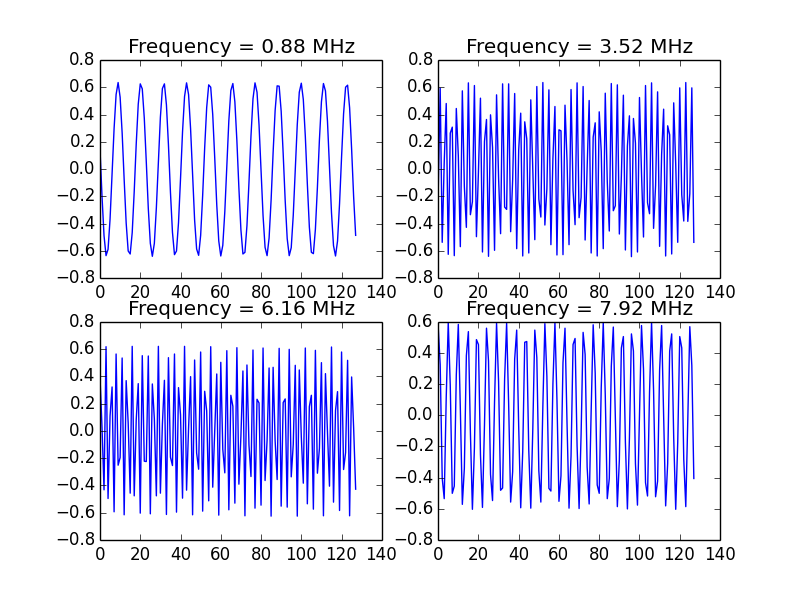
\includegraphics[scale=0.7]{sampling_time.png}
\caption{Time domain effects of changing the ratio between the input frequency and the sampling frequency.}
\label{fig:sampling_time}
\end{figure}

Although the input to the sampler was a pure sinusoid, all but the lowest frequency output appears to have additional aliased frequency components.  This can be explained by the Nyquist-Shannon sampling theorem.  Sampling a continuous time signal can be interpreted as multiplying it by an impulse train, a sum of periodically delayed delta functions, in the time domain.  This multiplication by a signal that is zero only at regular intervals will result in the sampled version of the original continuous time signal. The Fourier transform of the impulse train will be a sum of evenly spaced complex exponentially. The multiplication by the impulse train in the time domain corresponds to a convolution in the frequency domain, therefore creating "copies" of the original continuous time spectrum.
    The additional frequencies can be explained by the phenomenon known as aliasing, in which the aforementioned shifted "copies" of the spectra resulting from the convolution in the frequency domain, overlap with each other. Figure \ref{fig:aliasing} illustrates this concept. 
    
\begin{figure}[h!]
\centering
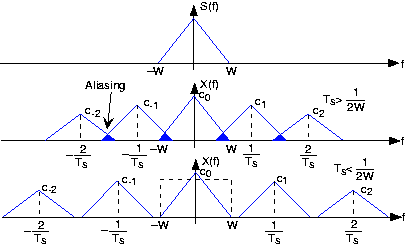
\includegraphics[scale=0.7]{alias_eg.png}
\caption{An illustration of aliasing in the frequency domain. The overlapping parts of the signal prevent perfect reconstruction from the sampled representation.}
\label{fig:aliasing}
\end{figure}

The spectra of the measured signals are shown in Figure\ref{fig:sampling_f}.

\begin{figure}[h!]
\centering
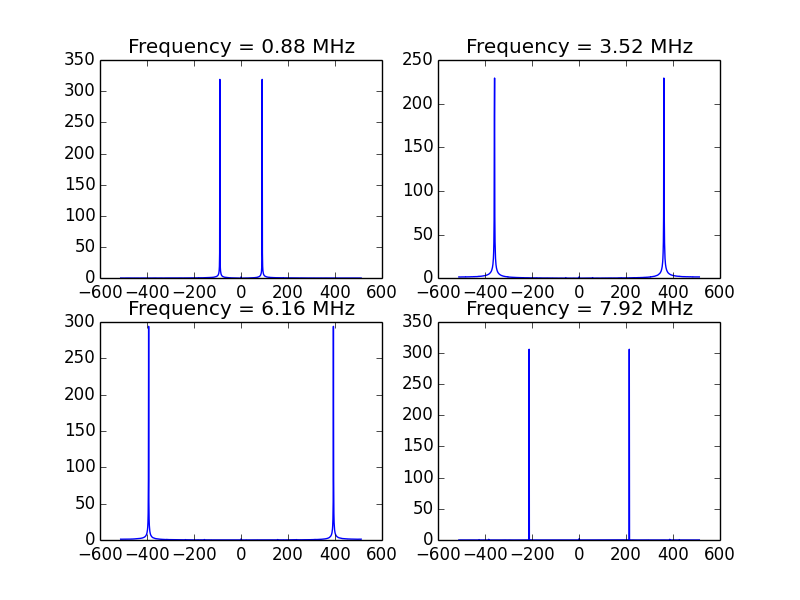
\includegraphics[scale=0.7]{sampling_f.png}
\caption{Frequency domain effects of changing the ratio between the input frequency and the sampling frequency.}
\label{fig:sampling_f}
\end{figure}

The same effects can be observed when attempting to sample signals at significantly lower rates than required by the Nyquist sampling theorem as shown in \ref{fig:sampling_f_ext}. Sampling at the Nyquist frequency does not result in aliasing in this case as for the pure sinusoids of our input the spectra do not overlap.

\begin{figure}[h!]
\centering
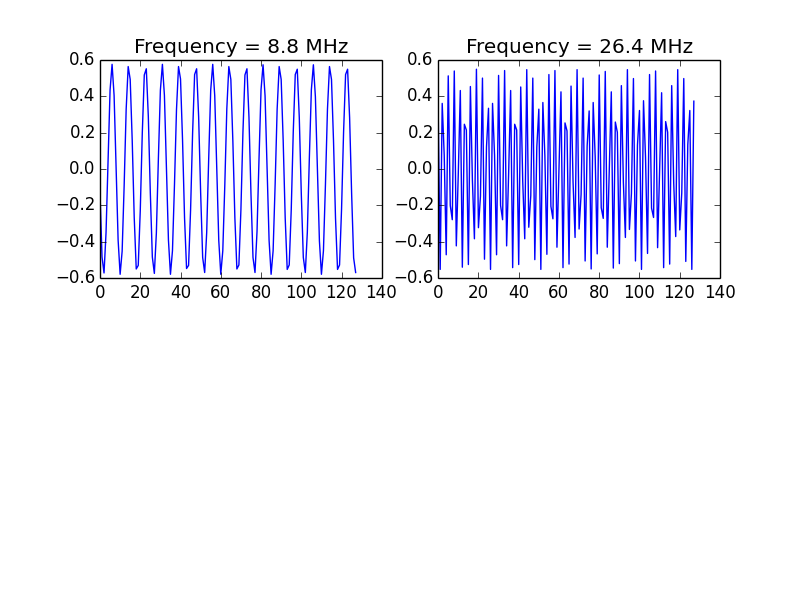
\includegraphics[scale=0.7]{sampling_time_ext.png}
\caption{Time domain effects of changing the ratio between the input frequency and the sampling frequency.}
\label{fig:sampling_f_ext}
\end{figure}

  A closer look at \ref{fig:sampling_f_ext} shows that this plot is not the perfect delta function we would mathematically expect; we notice that there are more frequencies than just the single the tone, however they decay quickly and are significantly smaller than the main component.  This shape arises from the nature of discrete signals. Taking only $N$ samples of the signal is in effect the same as multiplying the input signal by a rectangular window in in the time domain.  If we analyze the effect of this window function in the frequency domain, we notice that a rectangular window becomes a sinc function.  A sinc function has most of its energy concentrated in the "main lobe" and "side lobes" that decay in amplitude over time. In short this noise is inherent to converting a continuous representation to a discrete one and is known as spectral leakage.  In order to minimize these effects we can use different types of window functions such as Kaiser windows, which are optimized for their ratio between their main lobe and side lobe amplitudes. 
  There are other effects of discretizing the signal as well. As previously explained the DFT corresponds to samples of the DTFT.  For an $N$ point DFT, the spacing of the frequencies represented by the samples is $\frac{2\pi}{}$.  This intuitively makes sense as the highest frequency a discrete time signal can have is $\pi$, meaning the value changes on every sample.
  
%  \begin{lstlisting}[frame=single]
%  sampling frequency 8.8MHz
%  1Vpp
%  factor | period
%  a .1 | 1.136us +/-0.4
%  b .4 | 284ns +/- 2
%  c .7 | 162.5ns +/- 2
%  d .9 | 126.1ns +/- 0.6
%  e 1  | 113.6ns +/- 0.4
%  f 3  | 37.9ns +/- 0.4
%  1024 samples
%  \end{lstlisting}
  
  
% week 2
 
 
 
 
% clock = 200 MHz
% ~2000 samples
% tried low and high frequencies
%  explain FPGA
%  plot spectrum analog
%  filter out USB, ifft, show plot
%  
%  show fpga time domain and frequency, DSB, SSB
%  advantages of DSB, SSB, digital, analog
%   analog can't generate pefect tones
%  fixed point

  \subsection{Simple Double Sideband Mixer}
  We can plot the output of the analog mixer for the case of a frequency above and below the LO frequency as shown in \ref{fig:analog_dsb}.  The Fourier transform allows us to view the frequency content of the signal. We can see that the result of the modulation yields two distinct sections of the waveform in the frequency domain symmetric about the carrier frequency.
  
\begin{figure}[h!]
\centering
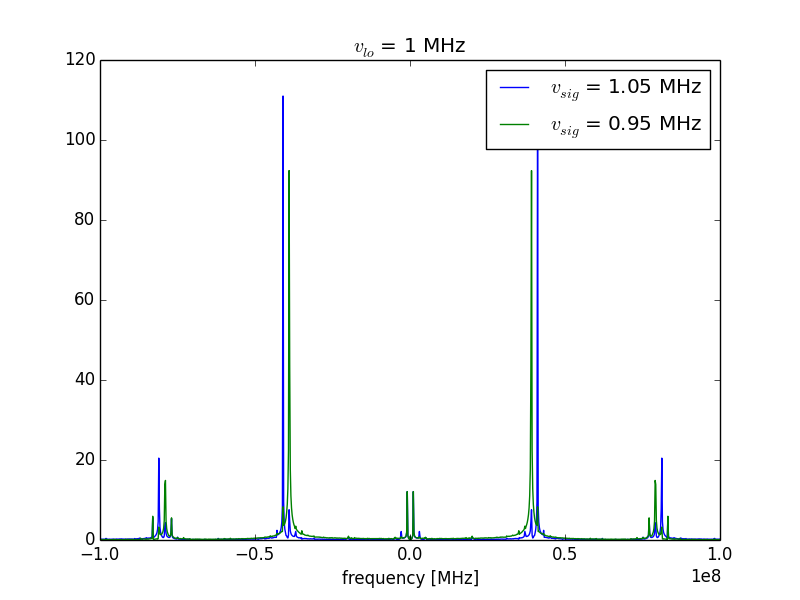
\includegraphics[scale=0.7]{analog_mix.png}
\caption{Output of the analog mixer for $v_{sig}$ values close to $v_{lo}$}
\label{fig:analog_dsb}
\end{figure}

  Because we can clearly see the difference between the upper and lower sidebands, and that these two sections of the are simply reflections of each other about the carrier frequency, we can use a filter to safely remove the upper sideband (USB) without any loss of information. In the frequency domain this is a particularly simple task as each of the coefficients $|f| \ge f_c$ can be multiplied by 0. The resulting spectrum and it's corresponding inverse transform showing the time domain signal are displayed in Figures \ref{fig:analog_filtered_f} \& \ref{fig:analog_filtered_t}.  
  
\begin{figure}[h!]
\centering
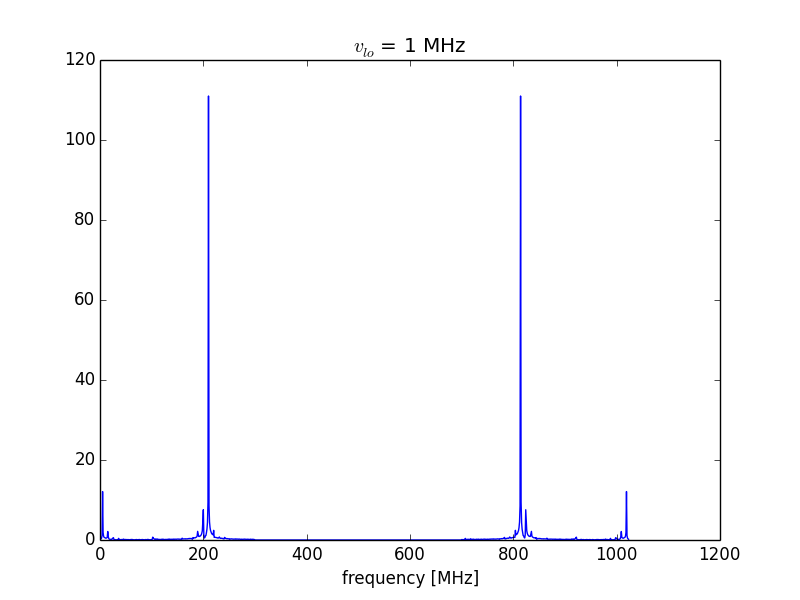
\includegraphics[scale=0.7]{analog_filtered_f.png}
\caption{Analog mixer output after filtering.}
\label{fig:analog_filtered_f}
\end{figure}

\begin{figure}[h!]
\centering
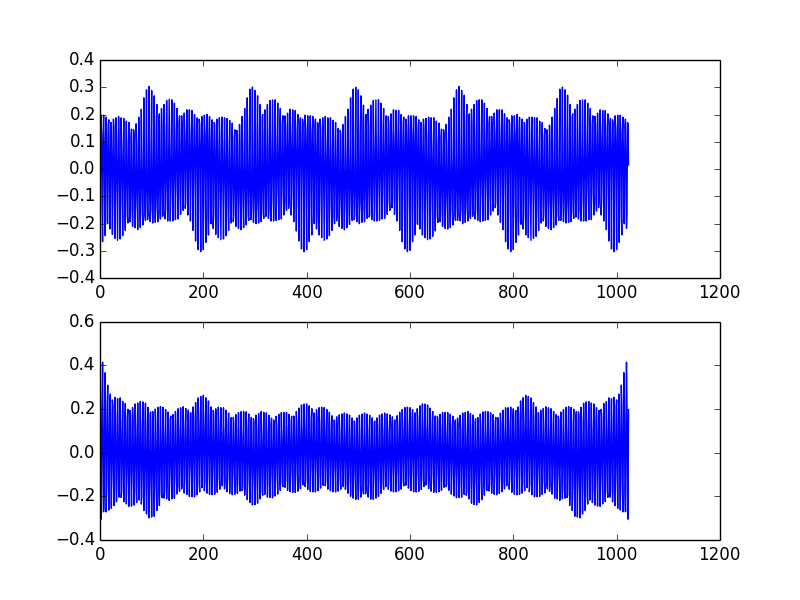
\includegraphics[scale=0.7]{analog_filtered_t.png}
\caption{Analog mixer output before and after filtering.}
\label{fig:analog_filtered_t}
\end{figure}

  \subsection{Digital Mixing on an FPGA}
  The result of applying the digital mixer on the ROACH are shown below.  Figure \ref{fig:digital_dsb} shows the same signals mixed before using the analog circuit.
  
\begin{figure}[h!]
\centering
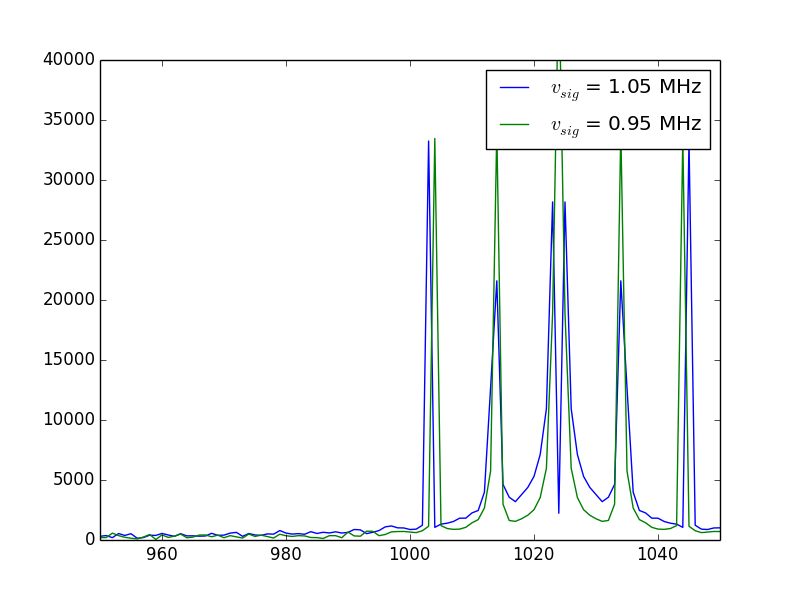
\includegraphics[scale=0.7]{digital_mix.png}
\caption{Output of the digital DSB mixer.}
\label{fig:digital_dsb}
\end{figure}

  We also analyzed the effect of summing the sine and cosine components to obtain the digital SSB output of the ROACH shown in \ref{fig:digital_ssb} 
\begin{figure}[h!]
\centering
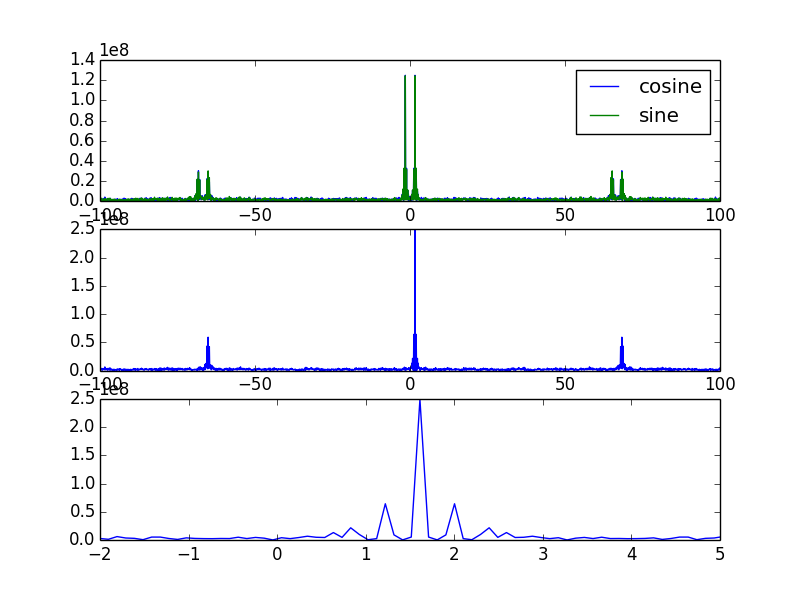
\includegraphics[scale=0.7]{ssb.png}
\caption{Output of the digital SSB mixer.}
\label{fig:digital_ssb}
\end{figure}

  We attempted to filter this signal, however a combination of what appears to be noise and spectral leakage introduced additional frequencies which are visible in the spectrum.  The effect of this on the time domain signal is that it is not the pure tone that we input as can be seen in \ref{fig:digital_ssb_t}
\begin{figure}[h!]
\centering
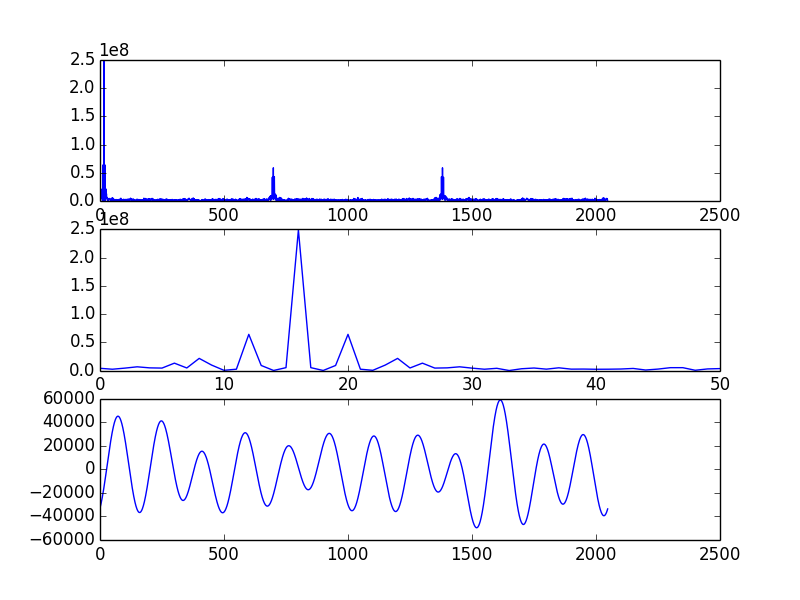
\includegraphics[scale=0.7]{digital_filtered.png}
\caption{Filtered digital SSB output.}
\label{fig:digital_ssb_t}
\end{figure}
  One of the major disadvantages of analog mixers is that they require very precisely matched sine and cosine signals. Digital I/Q mixing can use digital signals that are all synchronized to the same clock which can be used to ensure that these signals will actually be in perfect quadrature. This prevents phase noise in the IQ mixer. 
  
 $$ i(t) = cos(\omega_0 t) $$
 $$ I(e^{j\omega} = \frac{1}{2} \delta(\omega-\omega_0) + \frac{1}{2} \delta(\omega+\omega_0)$$
 $$ q(t) = jsin(\omega_0 t + \phi]{}) $$
 $$ Q(e^{j\omega} = \frac{e^{j\phi}}{2} \delta(\omega-\omega_0) - \frac{e^{-j\phi}}{2} \delta(\omega+\omega_0)$$
 $$ I + Q = \frac{1}{2} [\delta(\omega-\omega_0)(1+e^{j\phi}) - \delta(\omega+\omega_0)(1-e^{-j\phi})]$$
 
  As shown, the phase offset for one term will cause the imaginary components to not cancel out as expected.  An additional advantage to a digital filter implementation on an FPGA is that it allows easy addition of additional functionality. One example of additional processing in the case of oversampling the input would be the use of a decimation filter to improve SNR. The main advantage of analog mixer implementations is that for very high frequencies (on the order of GHz) such mixers can be much more cost effective to buy an analog mixer than an ADC that can sample the output at above the Nyquist rate.
  When comparing SSB and DSB, we can see that both sidebands encode the same information.  We can prove this based on the properties of the Fourier transform, as real valued signal such as the one we used for input must have an even spectrum in the frequency domain.  Because the result of mixing with a pure tone is a shifted version of our original spectrum, it will still be symmetric about some value and we only need one of the sidebands to represent the content of the original signal.  Using single sideband allows one to reduce the bandwidth required for transmitting AM radio signals and is therefore often the preferred method of transmission. Single sideband also requires less power, which is also a desirable property in transmitters.
  
  \subsection{Digital Down Converter}
  In order to remove the high frequency components we applied a low pass filter to this signal. We created this filter by taking 5 points in the frequency domain:
  $$H(k) = [1, 1, 1, 0, 0, 0, 1, 1]$$
Next we used python to take the inverse FFT to obtain the impulse response $h[n]$ which had the following coefficients:
$$h[n] = [0.125, -0.0518, -0.125, 0.302, 0.625, 0.302, -0.125, -0.0518]$$
After determining the impulse response of the filter, we can take the DFT again to see the effect of truncating the impulse response. Figure \ref{fig:lpf} shows the ideal low pass filter, the sampled FIR approximation, and the measured response.
\begin{figure}[h!]
\centering
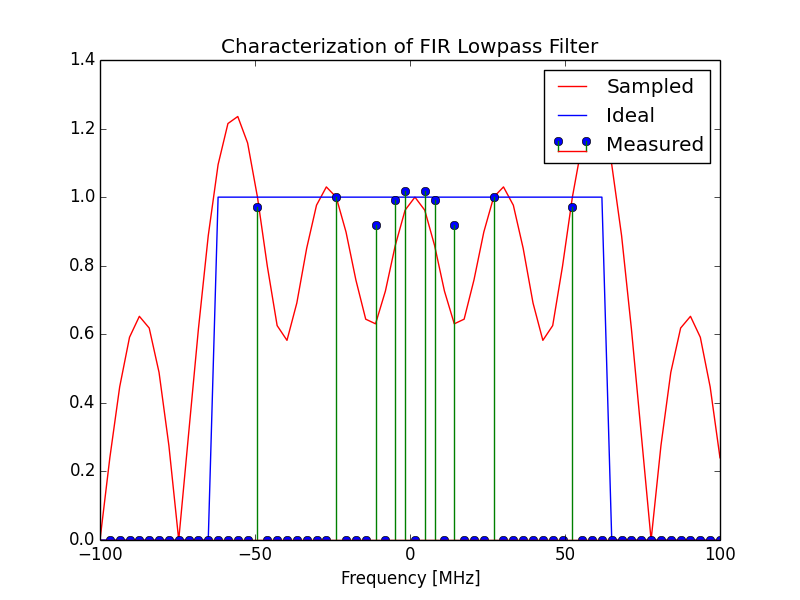
\includegraphics[scale=0.5]{lpf.png}
\caption{Comparison of ideal and implemented filter.}
\label{fig:lpf}
\end{figure}
  By multiplying the spectrum of our signal in the frequency domain by this filter, we attenuated high frequencies as the response of the filter is of a significantly lower amplitude at this point. Although our original goal was a box, the discontinuity in this function makes its impulse response infinite in the time domain. In order to implement the filter on the FPGA we took 8 samples of the ideal sinc function representing the filter.  The effect of the sampling on the frequency response became much more clear after taking the 64 point DFT of the 8 sample impulse response.  The 64 point DFT provides better resolution in the frequency domain with each point of the DFT corresponding to a division of $\frac{2\pi}{64}=\frac{\pi}{32}$.  The oscillations in the passband of the filter shown in Figure \ref{fig:lpf} illustrate the Gibbs phenomenon (the oscillations observed when attempting to approximate a discontinuous frequency response).
  In order to apply these coefficients to the FPGA we first had to convert them to a fixed point representation.
%!!!!!!!!!!!!!!!!!!!!!!!! TODO fixed point
We applied these coefficients to the registers in "reverse order" as the convolution operation implemented by the FPGA requires that the impulse response be "flipped" and shifted across the input signal. This made little difference in the case of the sinc function however as the function is symmetric and the coefficients would have been the same with the exception of the last one regardless of order.
  Although the filter was not ideal, we characterized the actual response by applying sinusoids of different frequencies and measuring the amount by which they were attenuated. Figure \ref{fig:lpf} shows that the measured amplitude of the signals, determined by the ratio of the root mean squared (RMS) input to output voltage, showed a reasonably good approximation of the 8 point sinc we intended to use. This plot was already normalized as the passband was designed not to attenuate input signals of frequencies within the passband.  As shown there was some attenuation and amplification of frequencies in the passband due to the oscillations resulting from the 8 point FIR approximation, the magnitude of the response is approximately 1.
  
%=======================================================================================  

\section{Conclusion}
  This series of lab experiments developed both a conceptual and practical understanding of digital signal processing systems and culminated in a functional design filter design. The basic concepts of sampling and Fourier Analysis are essential to data collection in almost any science or engineering field and the design of a digital down conversion system required both a strong understanding of signals and systems theory as well as the practical aspect of implementing a design on an FPGA. The mathematics and theory developed to complete these lab experiments is very generally applicable and perhaps the most important part of the lab itself; however the implementation of these concepts and understanding the non-idealities of implementing these concepts such as spectral leakage and the Gibbs phenomenon were also valuable learning experiences.
  
Code and results are available online at: https://github.com/viyer/astro121


\bibliographystyle{plain}
\bibliography{references}
\end{document}
